\section{Modelling the MW}
\begin{table}[H]\label{tab:models}
%\begin{center}
\begin{scriptsize}
\begin{tabular}{c c c c c }
\hline
Component  &  Besla07 &  LM2010 & Roeland12 & Gomez15 \\
\hline
Disk Model & Miyamoto-Nagai   & Miyamoto-Nagai &  &  \\
Disk Mass($M_{\odot}$) & $5.5^{10}$  & $1.0 \times 10^{11}$ & & \\
Disk Param & $R_d = 3.5$, $z=r_{disk}/5.0$  & $\alpha=1$, $a=6.5 kpc$, $b=0.6 kpc$ & &, $a=6.5kpc$, $b=0.26Kpc$\\
Bulge Model & Hernquist & Hernquist &  & Hernquist\\
Bulge Mass($M_{\odot}$) & $10^{10}$  &$3.4 \times 10^{10}$ & & \\
Bulge Param & $0.6 kpc$ &  $c=0.7kpc$  & $0.6Kpc$ &\\
DM halo Model & NFW  & Triaxial \ref{sec:LM10}  & Hernquist(NFW) & \\
DM halo mass($M_{\odot}$) & $10^{12}$ &$ \times 10^{10}$ & & \\
Halo Param & $c=11, r_{vir} = 258Kpc$& $r_{halo} = 12 Kpc$ & &\\
Solar distance $R_{\odot}$ (kpc) & 8.0 & 8.0  & & \\
reference &\href{http://adsabs.harvard.edu/abs/2007ApJ...668..949B}{Besla07} & \href{http://bit.ly/1fXtla9}{LM2010} & &  \\
\hline
\end{tabular}
\end{scriptsize}
%\end{center}
\end{table}




\begin{figure}[H]\label{MWBesla07}
\centering
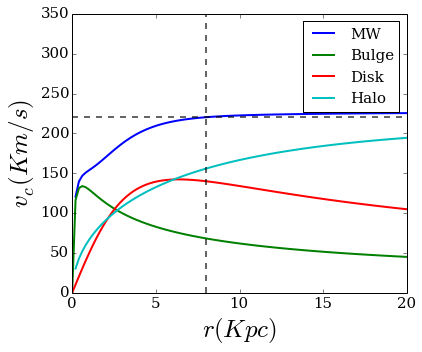
\includegraphics[scale=0.7]{../figures/MWBEsla07.png}
\end{figure}



\begin{figure}[H]\label{MWLM10}
\centering
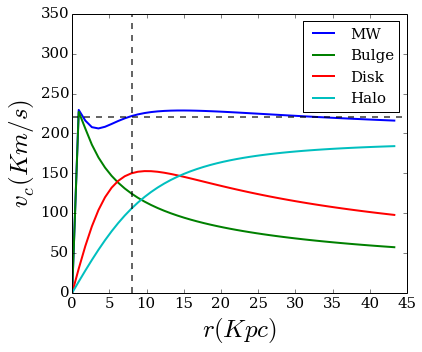
\includegraphics[scale=0.7]{../figures/MWLM10.png}
\end{figure}


